\lecture{31}{25 Mar. 10:00}{Cellular Homology}


\begin{example}
	Consider the composition of the quotient maps below $S^n \to \RP^n \to \RP^n/\RP^{n - 1} \cong S^n$. We want to compute the degree of this map.

	Note that this restricts to a homeomorphism on each component of $S^n \setminus \text{equator}$ as a map to $\RP^n \setminus \RP^{n - 1}$. Suppose we've oriented our copies of $S^n$ in such a way that the homeomorphism on the top hemisphere is orientation-preserving. The homeomorphism on the bottom hemisphere is given by taking the antipodal map and composing with the homeomorphism of the top hemisphere
	\begin{align*}
		\deg = \deg(\Id) = \deg(\text{antipodal}) = 1 + (-1)^{n + 1} = \twodef{0}{n \text{ even}}{2}{n \text{ odd}}
	\end{align*}
\end{example}

\subsection{Cellular Homology}

Suppose that $X$ is a CW complex. Then $(X^n, X^{n - 1})$ is a good pair for all $n > 1$, and $X^n/X^{n - 1}$ is a wedge of $n$-spheres, one for each $n$-cell $e^n_\alpha$. Hence:
\begin{align*}
	H_k(X^n, X^{n - 1}) \cong \twodef{0}{k \neq n}{\langle e_\alpha^n \st e_\alpha^n \text{ is an $n$-cell} \rangle }{k = n}
\end{align*}
\begin{defn}\label{defn-cellular-chain-groups}
	The cellular chain complex of $X$ has chain groups $H_n(X^n, X^{n - 1})$ with $X^{-1} = \0$.

	The boundary maps are given as:
	\begin{align*}
		d_1 : H_1(X^1, X^0)            & \to H_0(X^0)                       \\
		\langle \text{1-cells} \rangle & \to \langle \text{0-cells} \rangle
	\end{align*}
	is the usual simplicial boundary map. FOr $n > 1$, the boundayr map:
	\begin{align*}
		d_n(e_\alpha^n) = \sum_\beta d_{\alpha\beta} e_\beta^{n - 1}
	\end{align*}
	where $d_{\alpha\beta}$ is the degree of the map:
	\begin{align*}
		\xymatrix@=1.5in{
		\partial e^n_\alpha = S^{n - 1}_\alpha \ar[r]^-{\text{attaching map}} & X^{n - 1}\ar[r]^-{\text{quotient by } X^{n-1}\setminus e^{n - 1}_\beta} & S^{n-1}_\beta
		}
	\end{align*}
	In pictures, this is given as:
	\begin{center}
		%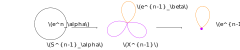
\includegraphics[scale=0.5]{cellular-boundary-map}
	\end{center}
\end{defn}

\begin{theorem}\label{thm-cellular-homology-coincides}
	The homology groups of the cellular chain complex (cellular homology groups) coincide with the singular homology groups.
\end{theorem}
